\documentclass[11pt]{article}

\usepackage{amsmath}
\usepackage{amssymb}
\usepackage[margin=0.68in]{geometry}
\usepackage{booktabs}
\usepackage{enumitem}
\usepackage{fancyhdr}
\usepackage{graphicx}
\usepackage[table]{xcolor}
\usepackage[hidelinks]{hyperref}
\usepackage{listings}
\usepackage{microtype}
\usepackage{tabularx}
\usepackage{titlesec}
\graphicspath{{docs/lessons/assets/}{../assets/}}

\definecolor{Ink}{gray}{0}
\definecolor{CodeGray}{gray}{0.96}
\hypersetup{
  hidelinks,
  pdftitle={ADK Lesson 031: Calibrated Analog Joystick},
  pdfauthor={Kevin Shanahan},
  pdfsubject={Two-axis calibration, center dead zones, explicit-time selection events, and circuit-native voltage evidence},
  pdflang={en-US}
}
\pagestyle{fancy}
\fancyhf{}
\lhead{\textsc{ADK Lesson 031}}
\rhead{Calibrated Analog Joystick}
\cfoot{\thepage}
\setlength{\headheight}{14pt}
\setlength{\parindent}{0pt}
\setlength{\parskip}{5pt}
\setlist{nosep,leftmargin=1.45em}
\titleformat{\section}{\Large\bfseries\color{Ink}}{\thesection}{0.5em}{}
\titleformat{\subsection}{\large\bfseries\color{Ink}}{\thesubsection}{0.5em}{}
\lstdefinestyle{adkcpp}{
  language=C++,
  backgroundcolor=\color{CodeGray},
  basicstyle=\ttfamily\small,
  keywordstyle=\color{Ink}\bfseries,
  commentstyle=\color{Ink},
  columns=fullflexible,
  keepspaces=true,
  showstringspaces=false,
  frame=single,
  rulecolor=\color{Ink},
  breaklines=true,
  tabsize=4
}
\newcommand{\checkbox}{\(\square\)}
\newcommand{\blank}[1]{\rule{#1}{0.4pt}}
\newcommand{\lessonbox}[1]{%
  \begin{center}\fcolorbox{Ink}{white}{\parbox{0.92\linewidth}{#1}}\end{center}}

\begin{document}

\begin{center}
  {\Huge\bfseries Calibrated Analog Joystick}\\[4pt]
  {\Large Preserve raw evidence, shape two axes, debounce one selection}\\[8pt]
  \textit{Three observations; one deterministic snapshot}
\end{center}

\begin{tabularx}{\linewidth}{@{}>{\bfseries}l X >{\bfseries}l X@{}}
Lesson & 031 --- component & Time & 150--210 minutes\\
Prerequisites & Lessons 002, 007, and 008 & Board & Arduino Mega 2560\\
Evidence & TP-X, TP-Y, RGB preview & Status & host verified; bench open\\
Energy class & E1: USB, passive joystick, resistor-limited RGB LED\\
\end{tabularx}

\lessonbox{\textbf{Specimen gate.} The official Elegoo manifests authorize a
``Joystick module'' family, not a universal pin order or catalog identity.
Before wiring, read the labels on the exact unpowered board and establish its
supply rating and signal roles. Do not infer KY-023, pin order, polarity, or
axis direction from board color or an internet photograph. Unknown markings
stop the physical procedure; they do not block the host lesson.}

\section{Mission and learning outcomes}

\[
\text{X raw + Y raw + switch raw}
\rightarrow\text{calibrated snapshot}
\rightarrow\text{RGB direction and magnitude}.
\]

By the end, you can:

\begin{itemize}
  \item distinguish raw ADC evidence from normalized position;
  \item map asymmetric travel around a measured center without floating point;
  \item explain why a center dead zone is not discarded evidence;
  \item debounce selection with caller-supplied time;
  \item predict initialization rollback and reverse-order shutdown;
  \item prove acquisition separately from input-mode safe state.
\end{itemize}

\section{Orientation and unpowered inspection}

\begin{center}
% ADK visual: pencil
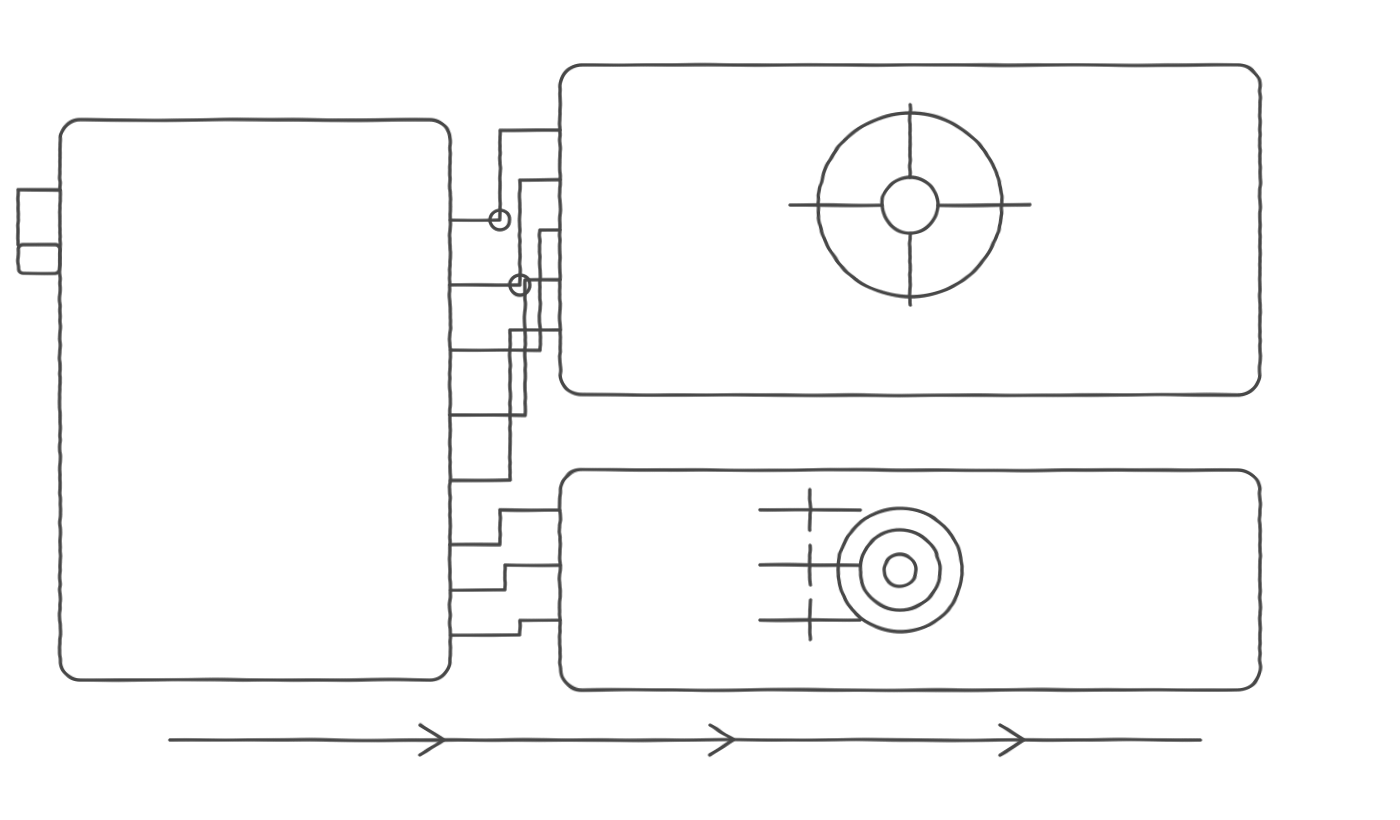
\includegraphics[width=0.96\linewidth]{031-analog-joystick-pencil.png}

\small\textit{Alternative text: monochrome orientation plate showing an
inspected joystick module connected to Mega A0, A1, D22, 5 V, and ground;
TP-X and TP-Y at the two analog signals; and a separately resistor-limited
common-cathode RGB LED on D5, D6, and D7.}
\end{center}

\begin{tabularx}{\linewidth}{@{}l l X@{}}
\toprule
Observed role & Reference pin & Connection after inspection\\
\midrule
X signal: VRx, X, or HOR & A0 / D54 & module signal; TP-X to Mega GND\\
Y signal: VRy, Y, or VER & A1 / D55 & module signal; TP-Y to Mega GND\\
select: SW, KEY, or SEL & D22 & switch-to-ground, internal pull-up\\
supply and common & 5 V and GND & only after rating and continuity checks\\
RGB preview & D5, D6, D7 & each pin through 330 \(\Omega\) to LED channel\\
\bottomrule
\end{tabularx}

\textbf{Unpowered checklist.}

\begin{itemize}
  \item[\checkbox] record every module label and its physical order;
  \item[\checkbox] continuity-check the ground terminal and select contact;
  \item[\checkbox] verify three separate RGB resistors and LED common polarity;
  \item[\checkbox] verify TP-X and TP-Y cannot contact 5 V or adjacent rows;
  \item[\checkbox] confirm no motor, relay, external supply, or unknown module.
\end{itemize}

Exact module/revision: \blank{2.0in}\quad Supply source/rating:
\blank{1.7in}.

\section{Calibration contract}

Each axis stores five facts: analog pin, observed minimum, center, observed
maximum, and dead-zone half-width. Valid calibration requires
\[
m<c<M,\qquad c-d>m,\qquad c+d<M.
\]
Here \(m\) is the observed minimum, \(c\) the center, \(M\) the observed
maximum, and \(d\) the dead zone. These are configured observations, not
claims about universal joystick travel.

\begin{equation*}
p(r)=
\begin{cases}
-1000\,\dfrac{c-d-r}{c-d-m}, & r<c-d,\\[6pt]
0, & c-d\le r\le c+d,\\[6pt]
1000\,\dfrac{r-(c+d)}{M-(c+d)}, & r>c+d.
\end{cases}
\end{equation*}

The implementation clamps before narrowing, uses 32-bit intermediates, and
applies inversion last. A raw value at or beyond an observed endpoint sets
\texttt{saturated}; it does not assert an electrical fault. Raw values remain
in the snapshot even when their normalized position is zero.

\subsection{Prediction worksheet}

Use \(m=80\), \(c=520\), \(M=960\), and \(d=40\).

\begin{tabularx}{\linewidth}{@{}r X X X@{}}
\toprule
Raw count & Region prediction & Position prediction & Saturated?\\
\midrule
80  & \blank{1.0in} & \blank{1.0in} & \blank{.8in}\\
479 & \blank{1.0in} & \blank{1.0in} & \blank{.8in}\\
480 & \blank{1.0in} & \blank{1.0in} & \blank{.8in}\\
560 & \blank{1.0in} & \blank{1.0in} & \blank{.8in}\\
561 & \blank{1.0in} & \blank{1.0in} & \blank{.8in}\\
960 & \blank{1.0in} & \blank{1.0in} & \blank{.8in}\\
\bottomrule
\end{tabularx}

\section{Lifecycle, ownership, and sample order}

Construction performs no hardware operation. Initialization validates both
axis configurations, three distinct pins, and Mega capabilities before
claiming X, then Y, then select. Any failure releases the claims from that
attempt in reverse order. Repeated successful initialization is inert.

Every \texttt{update(now)} reads X once, Y once, then delegates exactly one
select sample to the existing \texttt{Button}. Its snapshot contains raw and
calibrated axes, raw and debounced selection levels, press and release events,
and one complete status. Events remain stable until the next update.

\begin{lstlisting}[style=adkcpp]
const adk::Status status = joystick.update (now);
const adk::AnalogJoystickSnapshot view =
    joystick.snapshot ();

showJoystickPosition (view);
showSelectionEvent   (view);
\end{lstlisting}

Shutdown stops select, Y, then X. It preserves the last raw and interpreted
evidence. The retained snapshot reports a not-initialized status. The three
input endpoints return to \texttt{INPUT}; an RGB presenter is a separate owner
and must also be shut down by the sketch.

\section{Circuit-native presentation}

The RGB LED is not part of \texttt{AnalogJoystick}. The narrative sketch maps
the stable snapshot to an independent presentation:

\begin{itemize}
  \item a short blue pulse after all resources initialize proves acquisition;
  \item red intensity represents negative X, green intensity positive X;
  \item centered X uses blue at the same Y-derived brightness;
  \item Y scales the chosen direction's brightness;
  \item a debounced select event produces a brief all-channel marker.
\end{itemize}

The same color never carries the only distinction: TP-X and TP-Y retain direct
voltage evidence, and the lesson names the selected channel and magnitude in
text. Serial raw counts are optional supporting evidence.

\subsection{Current worksheet}

One 330 \(\Omega\) resistor is required per RGB channel. The sketch commands at
most one steady direction channel; the short event marker may command three.
A conservative zero-forward-voltage bound is
\[
I_{\mathrm{channel}}\leq\frac{5.0\ \mathrm{V}}{330\ \Omega}=15.2\ \mathrm{mA},
\qquad I_{\mathrm{RGB,total}}\leq45.5\ \mathrm{mA}.
\]
This is a design bound, not a measurement.

\begin{tabularx}{\linewidth}{@{}X l l X@{}}
\toprule
Quantity & Predicted & Measured & Interpretation\\
\midrule
TP-X at rest & within 0--5 V & \blank{.8in} & \blank{1.5in}\\
TP-Y at rest & within 0--5 V & \blank{.8in} & \blank{1.5in}\\
each RGB resistor & 330 \(\Omega\) & \blank{.8in} & \blank{1.5in}\\
select released/pressed & high / low & \blank{.8in} & \blank{1.5in}\\
\bottomrule
\end{tabularx}

\section{Narrative Mega example}

\begin{lstlisting}[style=adkcpp]
void loop ()
{
    const adk::TimePoint now (millis ());

    observeJoystick (now);
    decidePreview   ();
    showPreview     (now);
}
\end{lstlisting}

Objects appear in dependency order: Mega runtime, resource registry, joystick,
RGB endpoints, then presenter state. Setup reads as acquire, configure, start.
The loop reads as observe, decide, actuate. It takes one joystick snapshot and
never reads a pin directly.

\section{Predict, observe, interpret}

\begin{enumerate}
  \item With power absent, predict the center-region TP-X and TP-Y voltages and
        the select levels. Record the exact inspected pin labels.
  \item Apply USB power. Observe the blue acquisition pulse before interpreting
        any direction preview.
  \item Hold the stick at rest. Record raw counts and TP-X/TP-Y. Choose center
        and dead-zone values from repeated observations, not a single sample.
  \item Move X toward each mechanical limit without force. Compare raw count,
        normalized sign, direction channel, and TP-X.
  \item Repeat for Y and explain how Y changes magnitude without changing X
        direction.
  \item Bounce and hold select. Compare raw level, debounced level, and the
        single press/release events.
  \item Invoke shutdown. Observe RGB inactivity separately from all three input
        pins returning to their documented modes; then remove USB.
\end{enumerate}

\section{Diagnosis and stop conditions}

\begin{tabularx}{\linewidth}{@{}X X@{}}
\toprule
Observation & Stop, inspect, and interpret\\
\midrule
label or pin order differs & remove USB; follow the exact board, not this drawing\\
TP-X or TP-Y outside rails & remove USB; inspect supply, ground, and signal role\\
axes exchanged & correct role-to-pin configuration; do not rename raw evidence\\
rest drifts outside dead zone & repeat observations; do not hide faults with a huge zone\\
direction sign is opposite & use explicit inversion after confirming wiring\\
multiple selection events & inspect debounce trace and supplied timestamps\\
preview but no blue pulse & do not claim acquisition; inspect startup sequence\\
hot part or unstable USB & remove USB immediately; troubleshoot unpowered\\
\bottomrule
\end{tabularx}

\section{Exercises}

\begin{enumerate}
  \item Derive the two denominators for an asymmetric axis and explain why one
        global slope would bias the center.
  \item Identify every invalid configuration that can be rejected before a
        hardware read or claim.
  \item Draw the reverse rollback order when Y acquisition fails, then when
        select acquisition fails.
  \item Explain why \texttt{saturated} preserves evidence but cannot diagnose a
        short circuit.
  \item Treat the authorized tilt-ball family as an ordinary
        \texttt{DigitalInput} exercise. State why it does not justify a new
        semantic component.
\end{enumerate}

\section{Open hardware acceptance record}

\textbf{Software compilation and deterministic tests are not physical
results.} Leave every line blank until the named specimen and instrument are
actually used.

\begin{tabularx}{\linewidth}{@{}l X l X@{}}
\toprule
Board/revision & \blank{1.4in} & Commit & \blank{1.25in}\\
Joystick markings & \blank{1.4in} & RGB/resistors & \blank{1.25in}\\
Supply/instrument & \blank{1.4in} & Tool versions & \blank{1.25in}\\
Operator/date & \blank{1.4in} & Reviewer & \blank{1.25in}\\
\bottomrule
\end{tabularx}

\begin{itemize}
  \item[\checkbox] exact labels, pin order, voltage rating, continuity, and
        unpowered wiring recorded;
  \item[\checkbox] acquisition pulse predicted, observed, and interpreted;
  \item[\checkbox] TP-X and TP-Y center, both limits, and calibration recorded;
  \item[\checkbox] raw, normalized, centered, saturated, and inverted cases
        reconciled;
  \item[\checkbox] select bounce, press, release, and stuck state observed;
  \item[\checkbox] shutdown input modes and RGB inactivity established as
        separate evidence;
  \item[\checkbox] USB power-removal result recorded.
\end{itemize}

Prediction: \blank{5.8in}\\[8pt]
Observation: \blank{5.7in}\\[8pt]
Interpretation and limits: \blank{4.9in}

\lessonbox{\textbf{Stop rule.} Remove USB power for unknown markings,
uncertain pin order, an out-of-rail test point, missing resistor, wrong LED
polarity, unexpected behavior, a hot part, unstable power, or disagreement
between the schematic and breadboard. Do not move wiring while powered.}

\section{Reproduce the software evidence}

\begin{lstlisting}[style=adkcpp]
make analog-joystick-test
make host-test-exceptions
make arduino-Lesson031AnalogJoystick
make size-check
make lessons
make lessons-check
make site-check
make hardware-card LESSON=031 BOARD=mega2560
\end{lstlisting}

Record the exact AVR core, compiler, measured flash, and static RAM with the
canonical sketch. Re-measure when source or toolchain identity changes.

\section{Reference trail}

\begin{itemize}
  \item ADK \texttt{analog\_joystick.h}, \texttt{analog\_input.h},
        \texttt{button.h}, focused host tests, and canonical Lesson 031 sketch;
  \item ADK development, testing, safety, packaging, and PDF policies;
  \item the authorized Elegoo-set manifest for family provenance only;
  \item the exact module's markings and primary electrical source before
        powered work;
  \item Arduino Mega 2560 Rev3 datasheet for the board profile.
\end{itemize}

The searchable HTML reference is the primary accessible route. This printable
PDF uses real text, headings, lists, and monochrome graphics but does not claim
PDF/UA conformance.

\end{document}
